\documentclass[svgnames]{article}
\usepackage[utf8]{inputenc}
\usepackage{amsmath}
\usepackage{amssymb}
\usepackage{mathrsfs}
\usepackage{mathtools}
\newtheorem{mydef}{Given}
\newtheorem{mytheorem}{Theorem}
\usepackage{enumitem}
\usepackage{venndiagram}
\usepackage{smartdiagram}
\usepackage{caption}
\usepackage{subcaption}
%\usepackage[framed,numbered,autolinebreaks,useliterate]{mcode}
\usepackage{pgfplots}
%\usepackage{tkiz}
\usepackage{listings}
\definecolor{dkgreen}{rgb}{0,0.6,0}
\definecolor{gray}{rgb}{0.5,0.5,0.5}
\definecolor{mauve}{rgb}{0.58,0,0.82}
\usepackage{float}
\usepackage{graphicx}

\lstset{ %
  language=R,                     % the language of the code
  basicstyle=\footnotesize,       % the size of the fonts that are used for the code
  numbers=left,                   % where to put the line-numbers
  numberstyle=\tiny\color{gray},  % the style that is used for the line-numbers
  stepnumber=1,                   % the step between two line-numbers. If it's 1, each line
                                  % will be numbered
  numbersep=5pt,                  % how far the line-numbers are from the code
  backgroundcolor=\color{white},  % choose the background color. You must add \usepackage{color}
  showspaces=false,               % show spaces adding particular underscores
  showstringspaces=false,         % underline spaces within strings
  showtabs=false,                 % show tabs within strings adding particular underscores
  frame=single,                   % adds a frame around the code
  rulecolor=\color{black},        % if not set, the frame-color may be changed on line-breaks within not-black text (e.g. commens (green here))
  tabsize=2,                      % sets default tabsize to 2 spaces
  captionpos=b,                   % sets the caption-position to bottom
  breaklines=true,                % sets automatic line breaking
  breakatwhitespace=false,        % sets if automatic breaks should only happen at whitespace
  title=\lstname,                 % show the filename of files included with \lstinputlisting;
                                  % also try caption instead of title
  keywordstyle=\color{blue},      % keyword style
  commentstyle=\color{dkgreen},   % comment style
  stringstyle=\color{mauve},      % string literal style
  escapeinside={\%*}{*)},         % if you want to add a comment within your code
  morekeywords={*,...}            % if you want to add more keywords to the set
} 


%\renewcommand{\theenumi}{\Alph{enumi}}
\newenvironment{amatrix}[1]{%
  \left(\begin{array}{@{}*{#1}{c}|c@{}}
}{%
  \end{array}\right)
}

\newenvironment{tolerant}[1]{%
  \par\tolerance=#1\relax
}{%
  \par
}


\pgfmathdeclarefunction{gauss}{2}{%
  \pgfmathparse{1/(#2*sqrt(2*pi))*exp(-((x-#1)^2)/(2*#2^2))}%
}


\title{Statistical Methods: Homework 3}
\author{Cameron McIntyre}
\date{\today}

\begin{document}

\maketitle

\section{11.2.18}
A graph of the luxury suite data in Question 8.2.5 suggests that the $xy$-relationship is linear. Moreover, it makes sense to constrain the fitted line to go through the origin, since $x = 0$ suites will necessarily produce $y = 0$ revenue.

\begin{enumerate}[label = \alph*.]
\item Find the equation of the least squares line, $y = bx$. (Hint: Recall Question 11.2.14.)
\item How much revenue would 120 suites be expected to generate?
\end{enumerate}

\subsection*{Answer:}
\begin{enumerate}[label = \alph*.]
\item
$$\sum x=545$$
$$\sum y=33.9$$
$$\sum x^2=54437$$
$$\sum xy=3329.4$$

So, using our formulas:
$$\frac{\sum xy}{\sum x^2}=\frac{3329.4}{54437}=.061$$

The constraint is the that $\beta_0=0$
So our equation is:
$$y=.061x$$
\item
Using x = 120.

$$y = .061*120 = 7.32$$
So revenue is projected at 7.32 million.
\end{enumerate}

\section{11.2.26}
 Among mammals, the relationship between the age at which an animal develops locomotion and the age at which it first begins to play has been widely studied. The table below lists “onset” times for locomotion and for play in eleven different species (46). Fit the data to the $y = ax^b$ model.

\begin{table}[H]
\centering
 \begin{tabular}{l c c} 
\hline 
\bf  & \bf  Locomotion &\bf Play Begins, \\
\bf Species & \bf  Begins, $x$ (days) &\bf $y$ (days) \\
\hline
\textit{Homo sapiens} & 360 & 90  \\
\textit{Gorilla gorilla} & 165 & 105  \\
\textit{Felis catus} & 21 & 21  \\
\textit{Canis familiaris} & 23 & 26  \\
\textit{Rattus norvegicus} & 11 & 14  \\
\textit{Turdus merula} & 18 & 28  \\
\textit{Macaca mulatta} & 18 & 21  \\
\textit{Pan troglodytes} & 150 & 105  \\
\textit{Saimiri sciurens} & 45 & 68  \\
\textit{Cercocebus alb.} & 45 & 75  \\
\textit{Tamaisciureus hud.} & 18 & 46  \\
 \hline
 \end{tabular}
\end{table}

\subsection*{Answer}
We take logarithms.
$$y=ax^b \leftrightarrow \ln(y) = \ln(a) + b \ln(x)  \leftrightarrow \hat{y} = \hat{a} +b \hat{x}$$
$$b=\frac{n\sum x_i*y_i-(\sum x_i)(\sum y_i)}{n(\sum x_i^2)-(\sum x_i)^2}=\frac{11*161.37 - 40.86*41.49}
{11*164.71-40.86^2}=0.5606$$
$$\hat{a}=\frac{\sum y_i} - b\sum x_i{n}=\frac{41.491 - 0.5606*40.86}{11}=1.6892$$
$$b=0.5606$$
$$a=e^{1.6892}=5.415$$
So our equation is:
$$\hat{y}=5.415*x^{0.5606}$$

\section{11.3.2}
The best straight line through the Massachusetts funding/graduation rate data described in Question 11.2.7 has the equation $y = 81.088+0.412x$,where s$ = 11.78848$. 

\begin{enumerate}[label=\alph*]
\item Construct a 95\% confidence interval for $\beta _1$.
\item What does your answer to part (a) imply about the outcome of testing $H_0: \beta_1 = 0$ versus $H_1: \beta_1 \neq 0$ at the $\alpha = 0.05$ level of significance?
\item  Graph the data and superimpose the regression line. How would you summarize these data, and their implications, to a meeting of the state School Board?
\end{enumerate}

\subsection*{Answer:}
\begin{enumerate}[label=\alph*]
\item Construct a 95\% confidence interval for $\beta _1$.
$$\sum x_i=360$$
$$\sum x_i^2=5365.08$$
$$\sum x_iy_i=31402$$
$$\sum y_i^2=188255.3$$
$$s=11.78848$$
$DF=26-2=24$ and $T_{.025,24}=2.0639$

$$C.I.=\big[\hat{\beta_1}-t_{.025,24}\frac{s}{\sqrt{\sum(x-\bar{x})^2}}, \hat{\beta_1}+t_{.025,24}\frac{s}{\sqrt{\sum(x-\bar{x})^2}}\big]$$
$$C.I.=\big[.412-2.0639\frac{11.78}{\sqrt{380.46}},.412+2.0639\frac{11.78}{\sqrt{380.46}}]$$
$$C.I.=\big[-.835,1.659]$$
\item What does your answer to part (a) imply about the outcome of testing $H_0: \beta_1 = 0$ versus $H_1: \beta_1 \neq 0$ at the $\alpha = 0.05$ level of significance?

The confidence interval contains 0 so we can accept $H_0$ and say that $\beta_1$ is not significantly different than 0.
\item  Graph the data and superimpose the regression line. How would you summarize these data, and their implications, to a meeting of the state School Board?
\begin{figure}
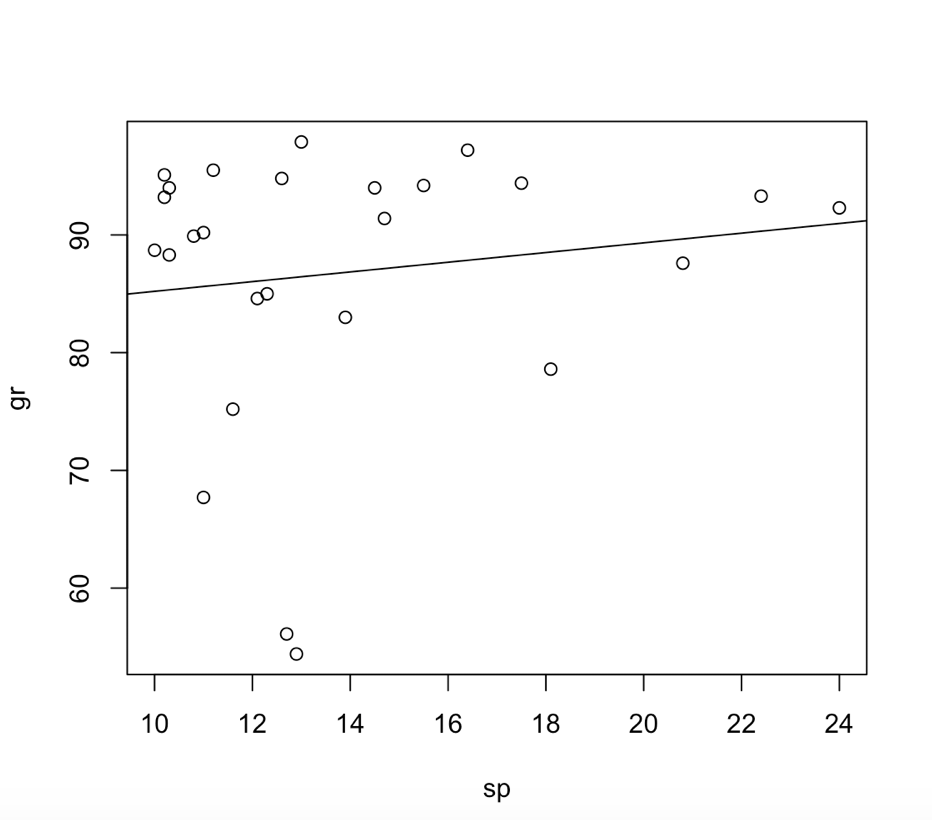
\includegraphics[width=\linewidth]{graph}
\caption{Data and Regression Line.}
\end{figure}
\newline
I would advise that state board that spending more money on students does not show a major boost in increasing the graduation rate. 
\end{enumerate}

\section{11.4.2}
Suppose that X and Y have the joint pdf $f_{X,Y}(x, y) = x + y, 0 < x < 1, 0 < y < 1$
Find $\rho(X,Y)$. 

\subsection*{Answer:}
$$\rho(x,y)=\frac{Cov(x,y)}{\sigma_x\sigma_y}$$
$$E[X]=\int_{0}^{1}\int_{0}^{1}x(x+y)dydx=\frac{7}{12}$$
$$E[Y]=\int_{0}^{1}\int_{0}^{1}y(x+y)dydx=\frac{7}{12}$$
$$E[XY]=\int_{0}^{1}\int_{0}^{1}xy(x+y)dydx=\frac{1}{3}$$
$$E[X^2]=\int_{0}^{1}\int_{0}^{1}y(x+y)dydx=\frac{5}{12}$$
$$E[Y^2]=\int_{0}^{1}\int_{0}^{1}y(x+y)dydx=\frac{5}{12}$$
Then we have,
$$Var[X]=E[X^2]-E[X]^2=\frac{5}{12}-\frac{49}{144}=\frac{11}{144}$$
$$Var[Y]=E[Y^2]-E[Y]^=\frac{5}{12}-\frac{49}{144}=\frac{11}{144}$$
$$Cov(X,Y)=E[XY]-E[X]E[Y]=\frac{1}{3}-\frac{49}{144}=\frac{-1}{144}$$

Finally,

$$\rho(x,y)=\frac{Cov(X,Y)}{(Var[X])^{\frac{1}{2}}(Var[Y])^{\frac{1}{2}}}=\frac{\frac{-1}{144}}{\frac{11}{144}}=\frac{-1}{11}$$

\section{11.5.4}
Suppose that the random variables X and Y have a bivariate normal pdf with $\mu_{X} = 56, \mu_{Y} = 11, \sigma^2_{X} = 1.2, \sigma^2_{Y} =2.6$, and $\rho = 0.6$. Compute $P(10 <Y<10.5 | x = 55)$. Suppose that n = 4 values were to be observed with x fixed at 55. Find $P(10.5 < \bar{Y} < 11 | x = 55)$. 
\subsection*{Answer:}

$$E[Y|x]=\mu_y +\frac{\rho \sigma_{y}}{\sigma_{x}}=11+\frac{.6*\sqrt{2.6}}{\sqrt{1.2}}(56-55)=10.11$$
$$Var[Y|x]=(1-\rho^2)\sigma^2=(1-.6^2)*2.6=1.664$$
Therefore,
$$P(10<y<10.5)=P(\frac{10-10.1}{1.289}<\frac{y-\mu_y}{\sigma_y}<\frac{10.5-10.1}{1.289})=P(-.09<z<.3)=.1538$$

And if there are 4 measurements (N=4):
$$P(10<\bar{y}<10.5)=P(\frac{10-10.1}{\frac{1.289}{2}}<\frac{y-\mu_y}{\frac{\sigma_y}{\sqrt{n}}}<\frac{10.5-10.1}{\frac{1.289}{2}})=P(.61<z<1.38)=.1871$$


\end{document}
